% !TeX root = ../main.tex
\section{连续映射}
\subsection{连续映射}
    \begin{Definition}[连续映射]
        设 $ X, Y $ 是拓扑空间, $ f: X\to Y $ 是映射, 若
        \begin{align*}
            \forall U\in \CN(f(x))\,\exists V\in\CN(x)\,(f(V)\subset U),
        \end{align*}
        则称 $ f $ 在 $ x $ 处\emph{连续}. 若 $ f $ 在 $ X $ 的每一点都连续, 则称 $ f $ 是 $ X $ 到 $ Y $ 的\emph{连续映射}.
    \end{Definition}

    \begin{Example}
        $ \id: X\to X $ 连续. 若 $ f: X\to Y $, $ g: Y\to Z $ 均连续, 则 $ g\circ f: X\to Z $ 连续. 
    \end{Example}

    \begin{Theorem}
        设 $ X, Y $ 是拓扑空间, $ f: X\to Y $ 是映射, 则以下条件等价:
        \begin{enumerate}
            \item $ f $ 是连续映射.
            \item $ \forall V\in\ST_{Y}\,(f^{-1}(V)\in \ST_{X}) $.
            \item $ \forall F\in\SF_{Y}\,(f^{-1}(F)\in \SF_{X}) $.
            \item $ \forall A\subset X\,(f(\bar{A})\subset\baro{f(A)}) $.
            \item $ \forall B\in\CB_{Y}\,(f^{-1}(B)\in\ST_{X}) $.
            \item $ \forall S\in\CS_{Y}\,(f^{-1}(S)\in\ST_{X}) $.
        \end{enumerate}
    \end{Theorem}
    \begin{Proof}
        $ (1)\Longrightarrow (2) $: 设 $ V $ 是 $ Y $ 的开集, 则 $ \forall x\in V\,(V\in\CN(x)) $, 由 $ f $ 连续
        \begin{align*}
            \exists U\in \CN(x)\,(f(U)\subset V)\Longrightarrow x\in U\subset f^{-1}(V),
        \end{align*}
        即 $ f^{-1}(V) $ 是开集.

        $ (2)\Longrightarrow (1) $: 对任意 $ U\in\CN(f(x)) $, 存在 $ V'\in\ST_{Y} $, 使得 $ f(x)\in V'\subset U $, 又因为 $ x\in f^{-1}(V')\in \ST_{X} $, 那么有 $ V:=f^{-1}(V')\in \CN(x) $, 于是 $ f(V)=f(f^{-1}(V'))=V'\subset U $, 即 $ f $ 是连续映射.

        $ (2)\Longrightarrow (3) $: 因为 $ f^{-1}(Y\sm A)=X\sm f^{-1}(A) $.

        $ (3)\Longrightarrow (4) $: $ f(A)\subset\baro{f(A)} $ 显然, 由 (3) 可知 $ A\subset f^{-1}(\baro{f(A)}) $, 而右侧是一个闭集, 两侧同时取闭包即有 $ \bar{A}\subset f^{-1}(\baro{f(A)}) $. 故 $ f(\bar{A})\subset\baro{f(A)} $.

        $ (4)\Longrightarrow (2) $: 设 $ V $ 是 $ Y $ 的开集, 由
        \begin{align*}
            f^{-1}(V)\subset X & \Longrightarrow f(\baro{f^{-1}(V)})\subset\baro{f(f^{-1}(V))}=\bar{V}\\
            & \Longrightarrow f^{-1}(\bar{V})\supset\baro{f^{-1}(V)},
        \end{align*}
        又由 $ \bar{V}\subset X $, 类似地, $ \baro{f^{-1}(\bar{V})}\subset f^{-1}(\bar{V}) $, 而 $ \baro{f^{-1}(\bar{V})}\supset f^{-1}(\bar{V}) $ 显然, 故 $ \baro{f^{-1}(\bar{V})}= f^{-1}(\bar{V}) $, 故 $ \baro{f^{-1}(V)}=f^{-1}(\bar{V}) $ 闭, 故 $ f^{-1}(V) $ 开. 

        $ (2)\Longleftrightarrow (5)\Longleftrightarrow (6) $ 显然.\qed
    \end{Proof}

    \begin{Example}[度量空间之间的连续映射]
        ~
        \begin{enumerate}
            \item 若 $ (X, d), (Y, \delta) $ 都是度量空间, $ f:X\to Y $ 是映射. 则 $ f $ 在 $ x_{0} $ 连续当且仅当
            \begin{align*}
                \forall \varepsilon>0\,\exists\delta>0\,(f(B(x_{0}), \delta)\subset B(f(x_{0}), \varepsilon)),
            \end{align*}
            即为 $ \varepsilon-\delta $ 定义. 
            \item 在 $ (X, d) $ 上定义点到集合的距离:
            \begin{align*}
                d(x, A)=\inf_{a\in A}d(x, a)
            \end{align*}
            与集合之间的距离
            \begin{align*}
                d(A, B)=\inf_{a\in A, b\in B}d(a, b),
            \end{align*}
            则对固定的 $ A $, 映射 $ d: X\to\R, x\mapsto d(x, A) $ 连续, 即证
            \begin{align*}
                \abs{d(x_{1}, A)-d(x_{2}, A)}\leqslant d(x_{1}, x_{2}).
            \end{align*}
            这因为
            \begin{align*}
                \forall a\in A\,(d(x_{1}, a)\leqslant d(x_{1}, x_{2})+d(x_{2}, a)), 
            \end{align*}
            故
            \begin{align*}
                d(x_{1}, A) & =\inf_{a\in A}d(x_{1}, a)\\
                & \leqslant d(x_{1}, x_{2})+\inf_{a\in A}d(x_{2}, a)=d(x_{1}, x_{2})+d(x_{2}, A),
            \end{align*}
            也即 $ d(x_{1}, A)-d(x_{2}, A)\leqslant d(x_{1}, x_{2}) $. 另一侧由对称性可证. 
            \item 由此:
            \begin{align*}
                \bar{A}=\set{x\in X: d(x, A)=0}.
            \end{align*}
        \end{enumerate}
    \end{Example}

    \begin{Theorem}[拼接定理]
        设 $ X $ 是拓扑空间, $ \set{X_{i}}_{i\in I} $ 是 $ X $ 的子集, 且 $ X=\bigcup_{i\in I}X_{i} $, 若 $ \forall i\in I, f_{i}:X_{i}\to Y $ 连续, 且 $ \forall i_{1}, i_{2}\in I\, \forall x\in X_{i_{1}}\cap X_{i_{2}}(f_{i_{1}}(x)=f_{i_{2}}(x)) $, 则定义
        \begin{align*}
            f(x)=f_{i}(x), \quad x\in X_{i}
        \end{align*}
        连续当且仅当下列其中一个成立
        \begin{enumerate}
            \item 对任意 $ i\in I $, $ X_{i} $ 是 $ X $ 的开子集,
            \item $ \abs{I}<\infty $, $ X_{i} $ 是 $ X $ 的闭子集.
        \end{enumerate}
    \end{Theorem}
    \begin{Proof}
        只证 (1). 因为
        \begin{align*}
            & \forall V\in\ST_{Y}\,\Big((f_{i}^{-1}(V)\in\ST_{X_{i}}\subset\ST_{X})\land (f^{-1}(V)=\bigcup_{i\in I}f_{i}^{-1}(V))\Big)\\
            \Longrightarrow{} & f^{-1}(V)\in\ST_{X}.
        \end{align*}
        即 $ f $ 连续. \qed
    \end{Proof}

    \begin{Example}
        设 $ f_{1}: [0, +\infty)\to \R, x\mapsto x $, $ f_{2}:(-\infty, 0]\to \R, x\mapsto -x $, 则作拼接
        \begin{align*}
            f(x)=\begin{cases}
                x & ,x\in[0, +\infty)\\
                -x & , x\in(-\infty, 0]
            \end{cases}
        \end{align*}
        即为 $ \R $ 上的连续函数 $ f(x)=\abs{x} $.
    \end{Example}

\subsection{同胚, 拓扑性质}
    \begin{Definition}[同胚]
        设 $ X, Y $ 是拓扑空间, $ f: X\to Y $ 是连续双射且 $ f^{-1} $ 连续, 则称 $ f $ 是 $ X $ 到 $ Y $ 的一个\emph{同胚}, 也称 $ X $ 与 $ Y $ 是\emph{同胚的}, 记作 $ X\cong Y $, 在同胚下保持不变的性质称为\emph{拓扑性质}.
    \end{Definition}

    \begin{Proposition}
        同胚关系是等价关系.
    \end{Proposition}

    \begin{Example}\label{ex:局部同胚不同胚}
        考虑映射
        \begin{align*}
            f: [0, 1)\to \T^{1},\quad t\mapsto \exp(2\pi \imag t),
        \end{align*}
        则 $ f $ 为连续双射, 但 $ f $ 不是同胚, 因为 $ f^{-1} $ 不连续, 例如 $ [0, 1/4) $ 在 $ f^{-1} $ 的原象不是 $ \T^{1} $ 的开集.

        \begin{minipage}[c]{.4\textwidth}
            \centering
            \vspace{1em}
            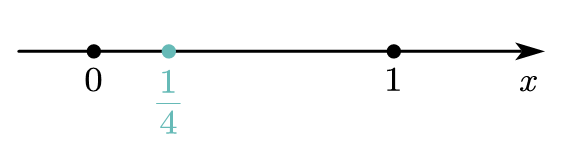
\includegraphics[width=6cm]{TopoFig1.png}
        \end{minipage}\quad
        \begin{minipage}[c]{.4\textwidth}
            \centering
            \vspace{.3em}
            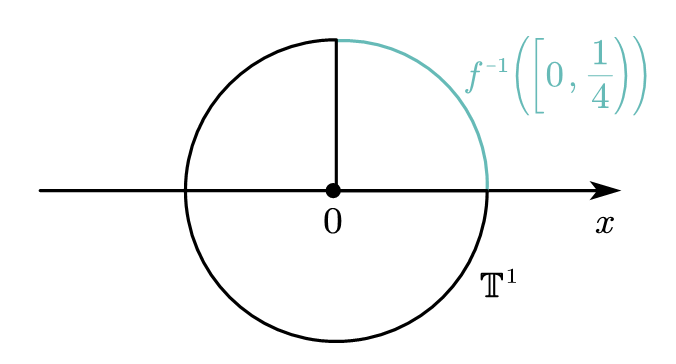
\includegraphics[width=6cm]{TopoFig2.png}
        \end{minipage}
    \end{Example}

    \begin{Example}
        设 $ C $ 是 $ \R^{n} $ 中有界闭凸集且包含内点, 则 $ C\cong \baro{\B^{n}}=\set{x\in\R^{n}:\norm{x}\leqslant 1} $, 其中 $ \baro{\B^{n}} $ 是 $ n $ 维闭单位球, 为此, 不妨 $ O\in C $ 为内点, 作 Minkowski 泛函:
        \begin{align*}
            p_{c}(x)=\inf\set{\lambda>0: \frac{x}{\lambda}\in C},
        \end{align*}
        则 $ C=\set{x\in\R^{n}:p_{c}(x)\leqslant1} $, 作同胚:
        \begin{align*}
            f:\baro{\B^{n}}\to c,\quad x\mapsto\begin{cases}
                \norm{x}/p_{c}(x)\cdot x & , x\neq 0,\\
                0 & , x=0.
            \end{cases}
        \end{align*}
        即可:
        \begin{center}
            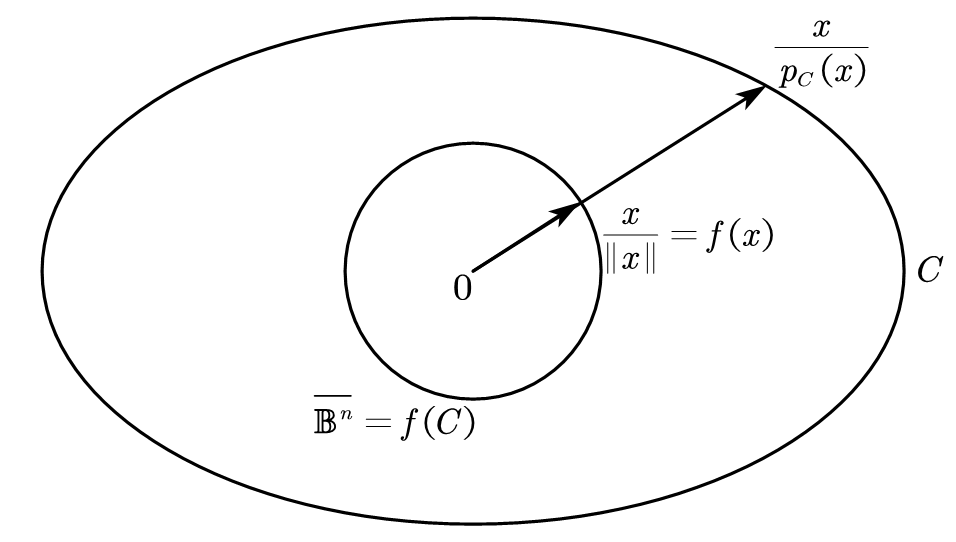
\includegraphics[width=9cm]{TopoFig3.png}
        \end{center}
    \end{Example}

    \begin{Example}
        ``刺破的球面'' $ \S^{n}\sm\set{p}\cong\R^{n} $, 其中 $ \S^{n}=\set{x\in\R^{n+1}:\norm{x}=1} $ 称为 $ n $ 维球面, $ p=(0, 0, \dots, 0, 1)\in \R^{n+1} $ 称为 $ \S^{n} $ 的北极, 考虑球极投影:
        \begin{align*}
            f: \S^{n}\sm\set{p}\to \R^{n}, \quad x\mapsto \frac{x-x_{n+1}p}{1-x_{n+1}},
        \end{align*}
        易验证 $ f $ 是同胚, $ f $ 可由以下方式导出. 

        对任意 $ x\in\S^{n}\sm\set{p} $, 引一条 $ x $ 与 $ p $ 的连线与赤道面 $ \R^{n}=\set{x\in\R^{n+1}: x_{n+1}=0} $ 交于 $ y $, 则
        \begin{align*}
            \begin{cases}
                y=\lambda x+(1-\lambda)p \\
                y_{n+1}=0,
            \end{cases}
            \Longrightarrow \lambda=\frac{1}{1-x_{n+1}},
        \end{align*}
        代入即解出 $ y $.
        \begin{center}
            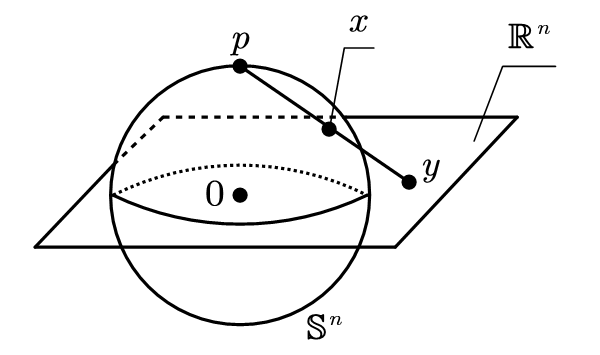
\includegraphics[width=7cm]{TopoFig4.png}
        \end{center}
    \end{Example}
    
    \begin{Example}
        称 $ \T^{2}=\T^{1}\times\T^{1} $ 是一个 2-- 环面, 则 $ \T^{2} $ 同胚于带柄的杯子, 在 $ \R^{3} $ 中 $ \T^{2} $ 可表示为
        \begin{align*}
            \T^{2}=\set{x\in\R^{3}:(\sqrt{x_{1}^{2}+x_{2}^{2}}-a)^{2}+x_{3}^{2}=1},\quad a>1,
        \end{align*}
        即 $ x_{1}x_{3} $ 平面上圆周 $ (x_{1}^{2}-a)^{2}+x^{3}=1, x_{2}=0 $ 绕 $ x_{2} $ 轴旋转而得.
        \begin{center}
            \includegraphics[width=6cm]{example-image-a}
        \end{center}
    \end{Example}

    \begin{Definition}[局部同胚]
        设 $ X, Y $ 为拓扑空间, $ f: X\to Y $ 连续, 若
        \begin{align*}
            \forall x\in X\,\exists U\in\CN(x)(f(U)\in\ST_{Y})
        \end{align*}
        且 $ f:U\to f(U) $ 是同胚, 则称 $ f $ 是\emph{局部同胚}.
    \end{Definition}
    同胚必为局部同胚, 但反之不成立, 例如例 \ref{ex:局部同胚不同胚} 中提到的
    \begin{align*}
        f: [0, 1)\to \T^{1},\quad t\mapsto \exp(2\pi \imag t).
    \end{align*}

    \begin{Definition}[不动点性质]
        设 $ X $ 是拓扑空间, $ f: X\to X $ 是连续映射, 若
        \begin{align*}
            \forall f: X\to X\, \exists \Star{x}\in X\,(f(\Star{x})=\Star{x}),
        \end{align*}
        则称 $ X $ 具有\emph{不动点性质}. 
    \end{Definition}
    可以此判断拓扑空间不同胚, 例如 $ \mathbb{I}=[0, 1],\ \T^{1}=\set{z\in\C: \abs{z}=1} $, 因为 $ \mathbb{I} $ 有不动点性质, 但 $ f: \T^{1}\to \T^{1}, z\mapsto -z $ 没有不动点, 故 $ \mathbb{I} $ 与 $ \T $ 不同胚. 